\def\retinafocusinference{
    Với sự xuất hiện của nhánh tập trung đối tượng\index{nhánh tập trung đối tượng}, mô hình RetinaFocus thay đổi chiến lược trong quá trình dự đoán, so với mô hình RetinaFace, giúp xử lý ảnh chất lượng cao một cách nhanh chóng và tiết kiệm chi phí tính toán hơn.
    Chiến lược trong quá trình dự đoán này được kế thừa từ nghiên cứu của mô hình AutoFocus \cite{najibi2019autofocus}.

    \noindent
    Cụ thể chiến lược trong quá trình dự đoán của mô hình RetinaFocus gồm các bước sau: \\
    - Bước 1: Với ảnh đầu vào có kích thước lớn, ta giảm kích thước của ảnh về kích thước đã được định sẵn từ trước. \\
    - Bước 2: Với ảnh kích thước nhỏ, ta đưa qua mô hình RetinaFocus và thu được hai đầu ra: hộp giới hạn\index{hộp giới hạn} (đầu ra của nhánh xác định đối tượng\index{nhánh xác định đối tượng})và khu vực cần tập trung\index{khu vực cần tập trung} (đầu ra của nhánh tập trung đối tượng\index{nhánh tập trung đối tượng}).
    Kết quả của hộp giới hạn\index{hộp giới hạn} sẽ được lưu lại để phục vụ cho thuật toán Focus Stacking.
    Kết quả khu vực cần tập trung\index{khu vực cần tập trung} sẽ được sử dụng cho các bước tiếp theo. \\
    - Bước 3: Kiểm tra xem có còn khu vực cần tập trung\index{khu vực cần tập trung} nào chưa được đưa qua mô hình RetinaFocus hay không.
    Nếu còn, vòng lặp tiếp tục, ta đi đến Bước 4.
    Nếu không còn, vòng lặp kết thúc, ta đi đến Bước 5. \\
    - Bước 4: Với mỗi khu vực cần tập trung\index{khu vực cần tập trung}, ta lấy được toạ độ của chúng trên ảnh đầu vào kích thước lớn và đưa những toạ độ này qua thuật toán sinh Focus Chip.
    Trong thuật toán này, ta sẽ định sẵn từ trước một giá trị ngưỡng tự tin\index{ngưỡng tự tin} và thuật toán sẽ giúp ta lựa chọn được những khu vực cần tập trung mà có độ tự tin\index{độ tự tin} của nhánh tập trung đối tượng\index{nhánh tập trung đối tượng} cao hơn so với ngưỡng tự tin\index{ngưỡng tự tin}.
    Từ đó, thuật toán Focus Chip đưa các khu vực này qua một số bước xử lý trước khi trả đầu ra là các khu vực trên ảnh cần được đưa qua mô hình RetinaFocus một lần nữa.
    Các khu vực trên ảnh này sau đó lại được thu nhỏ (hoặc phóng to tuỳ thuộc vào kích thước của khu vực đó trên ảnh đầu vào kích thước lớn) về kích thước đã được định sẵn từ trước.
    Sau đó, ta đưa các khu vực này quay trở lại Bước 2. \\
    
    \begin{figure}[H]
        \centering
        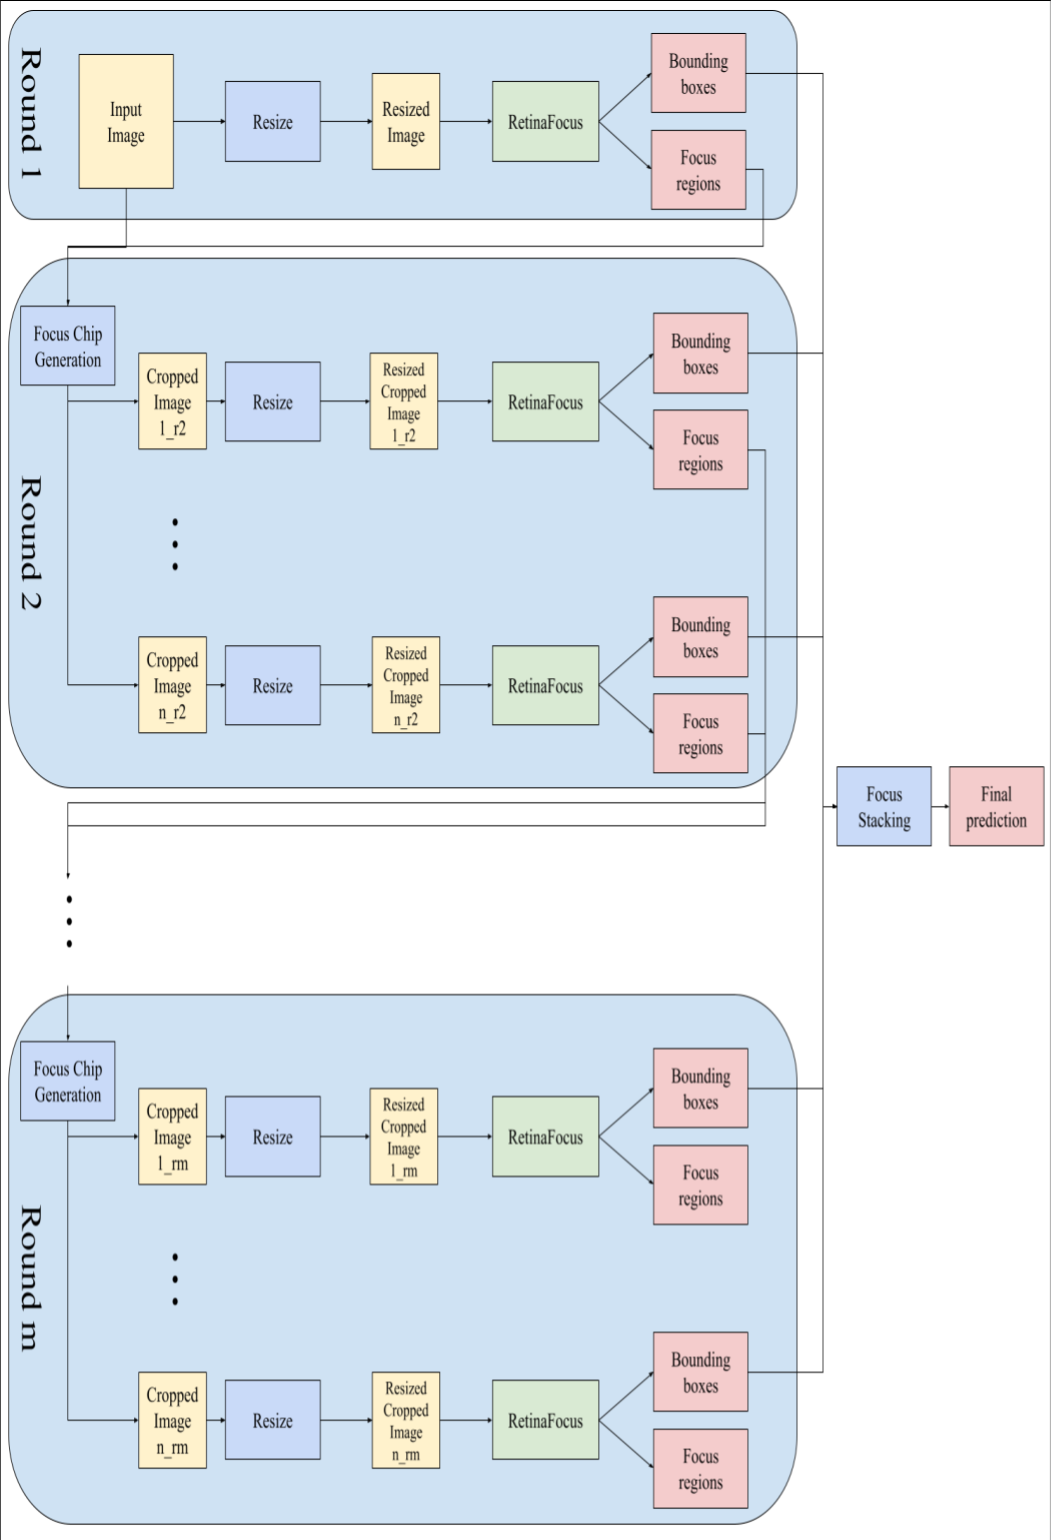
\includegraphics[width=15cm, trim={0.1cm 0.1cm 0.1cm 0.1cm}, clip] {images/retinafocus_infer_strategy}
        \caption{Sơ đồ mô phỏng chiến lược dự đoán của mô hình RetinaFocus}
        \label{fig:retinafocus_infer_strategy}
    \end{figure}
    
    \noindent
    - Bước 5: Ta tổng hợp lại các kết quả của các hộp giới hạn\index{hộp giới hạn} qua từng vòng lặp.
    Ta đưa các kết quả này qua thuật toán Focus Stacking để thu được kết quả dự đoán về hộp giới hạn\index{hộp giới hạn} cuối cùng của mô hình RetinaFocus và kết thúc quá trình dự đoán cho một ảnh đầu vào kích thước lớn.

    \noindent
    Với chiến lược trong quá trình dự đoán như trên, qua mỗi vòng lặp hay qua mỗi lần ta xử lý kết quả của nhánh tập trung đối tượng\index{nhánh tập trung đối tượng}, ta đều thay đổi kích thước của ảnh về giá trị kích thước đã được định sẵn từ trước, trước khi ta tiếp tục đưa qua mô hình RetinaFocus.
    Điều này giúp cho chiến lược dự đoán này có thể mô phỏng được kích thước của ảnh trong chiến lược Image Pyramids.
    Trong khi đó, việc thuật toán sinh Focus Chip cắt ảnh và loại bỏ bớt các khu vực không cần tập trung trên ảnh giúp chiến lược dự đoán này tiết kiệm được rất nhiều các pixels và giảm thiểu đáng kể chi phí tính toán và tăng tốc được quá trình dự đoán của mô hình.

    \begin{figure}[H]
        \centering
        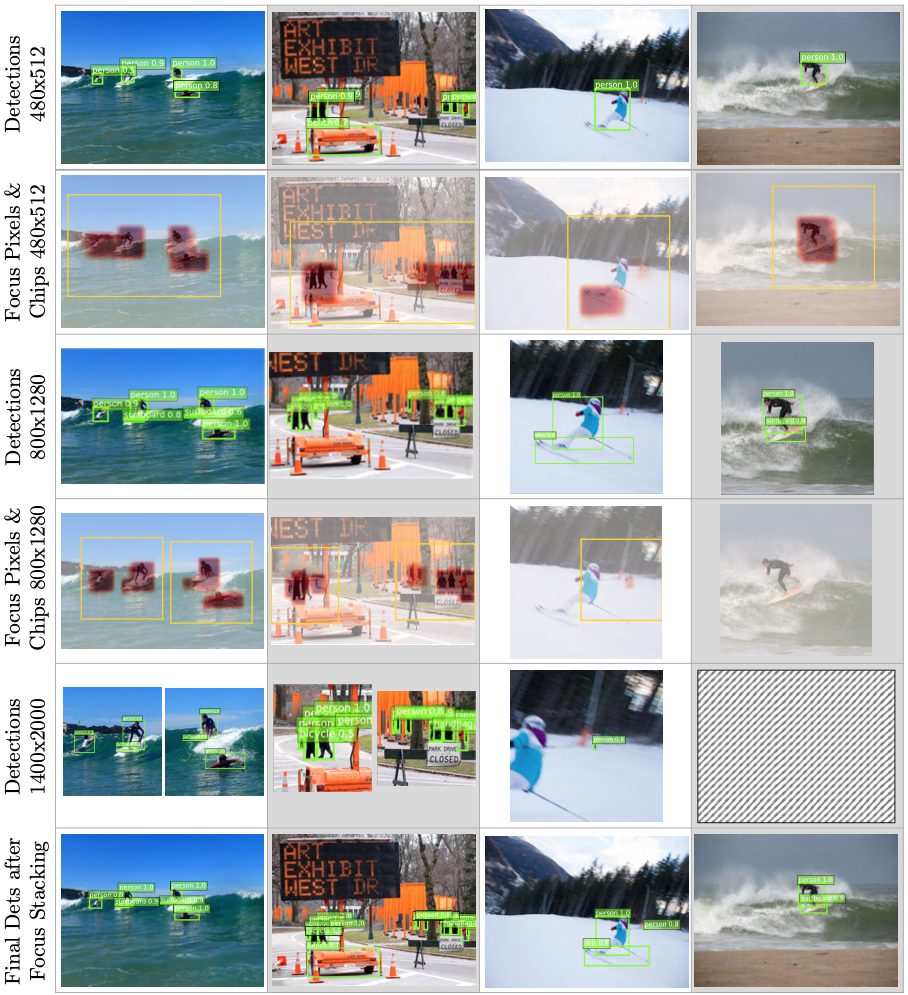
\includegraphics[width=15cm] {images/autofocus_results_3}
        \caption{Một số ví dụ về chiến lược dự đoán của mô hình AutoFocus (Nguồn: \cite{najibi2019autofocus})}
        \label{fig:autofocus_results_3}
    \end{figure}

    \noindent
    Chiến lược dự đoán trên mang lại cho ta nhiều giá trị cần được định sẵn từ trước và các giá trị này ảnh hưởng trực tiếp tới việc đánh đổi giữa độ chính xác và tốc độ dự đoán của mô hình.
    Cụ thể, với các kích thước ảnh được định sẵn làm kích thước đầu vào cho mô hình RetinaFocus, việc lựa chọn các kích thước ảnh đầu vào cho mô hình lớn sẽ giúp tăng độ chính xác của mô hình nhưng giảm tốc độ dự đoán và ngược lại, việc lựa chọn các kích thước ảnh nhỏ sẽ làm giảm độ chính xác của mô hình nhưng giúp tăng tốc độ dự đoán. \\
    Một tham số khác cũng ảnh hưởng đến việc đánh đổi này là ngưỡng tự tin\index{ngưỡng tự tin} của nhánh tập trung đối tượng\index{nhánh tập trung đối tượng}.
    Ngưỡng tự tin cao sẽ khiến mô hình sinh ra ít khu vực cần tập trung\index{khu vực cần tập trung}, từ đó độ chính xác sẽ giảm đi nhưng tốc độ được tăng lên.
    Ngược lại, ngưỡng tự tin thấp sẽ khiến mô hình sinh ra nhiều khu vực cần tập trung\index{khu vực cần tập trung}, từ đó độ chính xác sẽ tăng lên nhưng tốc độ được sẽ bị giảm đi đáng kể. \\
    Ngoài ra, ta cũng có thể lựa chọn tham số là số vòng lặp\index{số vòng lặp} của chiến lược dự đoán.
    Với số vòng lặp\index{số vòng lặp} ít, mô hình sẽ dự đoán ít đi giúp tốc độ được cải thiện nhưng độ chính xác sẽ bị ảnh hưởng và ngược lại, số vòng lặp\index{số vòng lặp} lớn sẽ khiến mô hình sẽ dự đoán nhiều lên, điều này khiến tốc độ chậm lại nhưng độ chính xác sẽ cao hơn. \\
    Chiến lược dự đoán này đòi hỏi ta cần phải tìm được bộ tham số phù hợp nhất và cân bằng nhất cho việc đánh đổi giữa độ chính xác và tốc độ dự đoán của mô hình.
}